\documentclass[11pt,a4paper]{memoir}\usepackage[]{graphicx}\usepackage[]{color}
%% maxwidth is the original width if it is less than linewidth
%% otherwise use linewidth (to make sure the graphics do not exceed the margin)
\makeatletter
\def\maxwidth{ %
  \ifdim\Gin@nat@width>\linewidth
    \linewidth
  \else
    \Gin@nat@width
  \fi
}
\makeatother

\definecolor{fgcolor}{rgb}{0.345, 0.345, 0.345}
\newcommand{\hlnum}[1]{\textcolor[rgb]{0.686,0.059,0.569}{#1}}%
\newcommand{\hlstr}[1]{\textcolor[rgb]{0.192,0.494,0.8}{#1}}%
\newcommand{\hlcom}[1]{\textcolor[rgb]{0.678,0.584,0.686}{\textit{#1}}}%
\newcommand{\hlopt}[1]{\textcolor[rgb]{0,0,0}{#1}}%
\newcommand{\hlstd}[1]{\textcolor[rgb]{0.345,0.345,0.345}{#1}}%
\newcommand{\hlkwa}[1]{\textcolor[rgb]{0.161,0.373,0.58}{\textbf{#1}}}%
\newcommand{\hlkwb}[1]{\textcolor[rgb]{0.69,0.353,0.396}{#1}}%
\newcommand{\hlkwc}[1]{\textcolor[rgb]{0.333,0.667,0.333}{#1}}%
\newcommand{\hlkwd}[1]{\textcolor[rgb]{0.737,0.353,0.396}{\textbf{#1}}}%

\usepackage{framed}
\makeatletter
\newenvironment{kframe}{%
 \def\at@end@of@kframe{}%
 \ifinner\ifhmode%
  \def\at@end@of@kframe{\end{minipage}}%
  \begin{minipage}{\columnwidth}%
 \fi\fi%
 \def\FrameCommand##1{\hskip\@totalleftmargin \hskip-\fboxsep
 \colorbox{shadecolor}{##1}\hskip-\fboxsep
     % There is no \\@totalrightmargin, so:
     \hskip-\linewidth \hskip-\@totalleftmargin \hskip\columnwidth}%
 \MakeFramed {\advance\hsize-\width
   \@totalleftmargin\z@ \linewidth\hsize
   \@setminipage}}%
 {\par\unskip\endMakeFramed%
 \at@end@of@kframe}
\makeatother

\definecolor{shadecolor}{rgb}{.97, .97, .97}
\definecolor{messagecolor}{rgb}{0, 0, 0}
\definecolor{warningcolor}{rgb}{1, 0, 1}
\definecolor{errorcolor}{rgb}{1, 0, 0}
\newenvironment{knitrout}{}{} % an empty environment to be redefined in TeX

\usepackage{alltt}

\usepackage[osf]{mathpazo}
\usepackage[mathcal,mathbf]{euler}
\usepackage{amsmath,amssymb,amsthm}
\usepackage[utf8]{inputenc}
\usepackage{graphicx,sidecap,tikz}
\usepackage{siunitx} 
\usepackage{marginnote}
\usepackage[breaklinks=true,colorlinks=true]{hyperref}

\usepackage[style=verbose-trad2,natbib=true]{biblatex}
\bibliography{dae}

% Version control
\immediate\write18{sh ./vc}
%%% This file has been generated by the vc bundle for TeX.
%%% Do not edit this file!
%%%
%%% Define Git specific macros.
\gdef\GITHash{7d26af967a77cf0297c0a8399d8e7d89ee73496d}%
\gdef\GITAbrHash{7d26af9}%
\gdef\GITParentHashes{d83783008f34c984f681d3152721e47e478d7891}%
\gdef\GITAbrParentHashes{d837830}%
\gdef\GITAuthorName{Christophe Lalanne}%
\gdef\GITAuthorEmail{ch.lalanne@gmail.com}%
\gdef\GITAuthorDate{2015-04-10 17:58:32 +0200}%
\gdef\GITCommitterName{Christophe Lalanne}%
\gdef\GITCommitterEmail{ch.lalanne@gmail.com}%
\gdef\GITCommitterDate{2015-04-10 17:58:32 +0200}%
%%% Define generic version control macros.
\gdef\VCRevision{\GITAbrHash}%
\gdef\VCAuthor{\GITAuthorName}%
\gdef\VCDateRAW{2015-04-10}%
\gdef\VCDateISO{2015-04-10}%
\gdef\VCDateTEX{2015/04/10}%
\gdef\VCTime{17:58:32 +0200}%
\gdef\VCModifiedText{\textcolor{red}{with local modifications!}}%
%%% Assume clean working copy.
\gdef\VCModified{0}%
\gdef\VCRevisionMod{\VCRevision}%


% To get lining figures in tables set by siunitx, which apparently uses the
% \mathrm font instead of \mathnormal
\SetMathAlphabet{\mathrm}{normal}{U}{eur}{m}{n}

\setSingleSpace{1.2}
\SingleSpacing

\setulmarginsandblock{1in}{1in}{*}
\setlrmarginsandblock{1in}{1in}{*}

\setheadfoot{\baselineskip}{\baselineskip} % headheight and footskip
\setheaderspaces{0.5in}{*}{*} % headdrop, headsep, and ratio

\checkandfixthelayout[lines]

% Set up custom headers and footers
\makepagestyle{stylish}
\copypagestyle{stylish}{headings}
\makerunningwidth{stylish}{5in}
\makeheadposition{stylish}{flushleft}{flushright}{}{}
\pagestyle{stylish}


\newcommand{\R}{\textsf{R}}
\newcommand{\marginlabel}[1] 
{\mbox{}\marginpar{\scriptsize \raggedright\hspace{0pt}#1}} 

\renewcommand*{\contentsname}{Table of Contents}
\setsecnumdepth{subsubsection}
\settocdepth{subsection}

\newcommand{\swelledrule}{%
    \tikz \filldraw[scale=.015,very thin]%
    (0,0) -- (100,1) -- (200,1) -- (300,0) --%
    (200,-1) -- (100,-1) -- cycle;}
\makeatletter
\makechapterstyle{grady}{%
    \setlength{\beforechapskip}{0pt}
    \renewcommand*{\chapnamefont}{\large\centering\scshape}
    \renewcommand*{\chapnumfont}{\large}
    \renewcommand*{\printchapternum}{%
        \chapnumfont \ifanappendix \thechapter \else \numtoName{\c@chapter}\fi}
    \renewcommand*{\printchapternonum}{%
        \vphantom{\printchaptername}%
        \vphantom{\chapnumfont 1}%
        \afterchapternum
        \vskip -\onelineskip}
    \renewcommand*{\chaptitlefont}{\Huge\itshape}
    \renewcommand*{\printchaptertitle}[1]{%
        \centering\chaptitlefont ##1\par\swelledrule}}
\makeatother
\chapterstyle{grady}


% Prevent page numbers from appearing on chapter pages
\aliaspagestyle{chapter}{empty}

\strictpagecheck % Turn on robust page checking
\captiondelim{} % Don't print a colon after "Figure #.#"


\usetikzlibrary{arrows,positioning,decorations.pathmorphing,trees}
\IfFileExists{upquote.sty}{\usepackage{upquote}}{}
\begin{document}

\frontmatter
\thispagestyle{empty}

\mbox{}\vspace{2in}
\noindent
\begin{flushright}
{\LARGE\itshape{}An}\hspace{1.5em}{\HUGE\scshape{}R Companion}\\[2\baselineskip]
{\LARGE\itshape{}to the}\hspace{1.5em}{\Huge\scshape{}Design and Analysis}\\[2\baselineskip]
{\LARGE\itshape{}of}\hspace{1.5em}{\Huge\scshape{}Experiments}
\end{flushright}

\vspace{6\baselineskip}
\hfill{\Large\scshape{}Christophe Lalanne}

\vfill
\begin{flushright}
  {\includegraphics[scale=.75]{logo}\\{\small \texttt{\GITAbrHash}}\\{\small %
    \texttt{\VCDateTEX}}}\par 
\vspace*{3\baselineskip}
\end{flushright}

\cleartorecto\tableofcontents*

\mainmatter



\section*{Foreword}


This document has been conceived as a supplemental reference material to
accompany the excellent book of Douglas C. Montgomery, \emph{Design and
Analysis of Experiments} (hereafter abbreviated as DAE). Now published in its
6th edition, this book covers numerous techniques used in the design and
analysis of experiments. This includes: Classical comparative experiments (two
groups of observations, independant or not), the natural extension to the case
of $k$ means to be compared (one-way ANOVA), various ways of blocking
(randomized blocks, latin squares and derived), the factorial-- in particular
the $2^k$ ones --and fractional designs, the fitting of regression models and
response surface methodology, a review of techniques for robust parameter
estimation, and the various derivation of standard design with fixed effects
(random factor, nested and split-plot designs).

Motivation for writting such a computer oriented document was initially
started when I was reading the document elaborated by Laura Thompson to
accompany Agresti's famous book, \emph{Categorical Data Analysis}\footnote{A
revised version of her textbook can be found here:
\href{https://home.comcast.net/~lthompson221/Splusdiscrete2.pdf}%
{https://home.comcast.net/~lthompson221/Splusdiscrete2.pdf}.}. Indeed, I found
that this really was a great idea as it brings to the other side of the
statistian's activity, that of computing. This document is somewhat different
of \texttt{splusdiscrete} since I don't pretend to be as exhaustive as she is
in her own manuscript.

While this textbook contains the same material as the original book written by
Montgomery, it is obviously not meant to be a partial electronic copy, nor to
be a complete replacement of the original book. Rather, I put some emphasis on
modern computer methods used to analyse data. Briefly, each chapter of this
textbook is organized as follow: first, I give a short summary of the main
concepts presented by Montgomery; then I try to illustrate some of the most
important (to my opinion!)  ones with \R. Exemples used by Montgomery are
completely re-analysed using \R. However, I do not answer to the proposed
exercices that can be found at the end of each chapter of DAE. I left them to
the interested reader, giving occasionnally some advice on ``\R\ way'' to do
the intended analysis.


\section*{About R}
\label{sec:about-r}
Montgomery mainly uses non-free software to analyse the dataset presented in
each chapter. Though these dedicated softwares have proved to be very good
packages for statistical analysis, their cost restrict their use to people
working in laboratory where specific credits are devoted to such
investment. Now, it seems that the avalailability of open-source software,
like \R, offers an elegant alternative to such solutions (often inaccessible
to students).
 
\R\ has been developed based on the \textsf{S} programming language and
\textsf{S-PLUS} software, although it is not a free completely rewritten clone
of \textsf{S-PLUS}. In fact, there are several differences between the two,
and the interested reader can refer to the following adress for a deeper
understanding of the way \R\ has been built: www.

\R\ can be freely downloaded on CRAN website
(\href{http://www.cran.r-project.org}{www.cran.r-project.org}), and many
documentation and tutorials can be found at the same address. What makes \R\ a
better choice to closed software like the ones Montgomery uses in his book is
that the source code of all the statistical built-in routines is available and
can be studied separately. In addition, users can add their own function to
suit their needs for a particular analysis, or for batching several analysis
process at once.

\section*{Exemple Scripts}
\label{sec:exemple-scripts}
All the analyses done by Montgomery in his book are replicated here
using \R, version 2.7, on Mac OS X though they were initiated with R
2.4 running on a Linux plateform. The source code for all the exemples
is available at the following address:
\begin{center} \href{http://www.aliquote.org/articles/stat/dae/}%
{www.aliquote.org/articles/stat/dae/}
\end{center} 
Datasets used in this textbook can also be found on this webpage. \R\
scripts should run without any problem with any version of \R\
$\geq2.0$. However, in case you encounter any problem, please send me
an email
(\href{mailto:christophe.lalanne@gmx.net}{christophe.lalanne@gmx.net})
with some detailed information on the bug found. I don't use
\texttt{Sweave} to process this document, because at the time of the
first writing of this textbook I felt more comfortable without it;
further, as there aren't any simulated data, nor too strong
packages dependency, a simple verbatim environment should be
sufficient for most of what I need. So all the included code is
static, except for some pieces of code in Chapter~2, and compilation relies on
\texttt{dvips} + \texttt{ps2pdf} only. Furthermore, I haven't splitted
the \texttt{tex} source into distinct chapters, so there is a ``huge''
source file that can be downloaded from there if anyone is interested
in getting the main \texttt{tex} file :
\href{http://www.aliquote.org/articles/stat/dae/}%
{www.aliquote.org/articles/stat/dae/dae.tex}. 

\chapter{Introduction}
\label{cha:introduction}
\pagenumbering{arabic}\setcounter{page}{1} 
The 6th edition of Montgomery's book, \emph{Design and Analysis of
Experiments}, has many more to do with the various kind of experimental
setups commonly used in biomedical research or industrial
engineering, and how to reach significant conclusions from the
observed results. This is an art and it is called the Design of
Experiment (\textsc{doe}). The approach taken along the textbook
differs from most of the related books in that it provides both a deep
understanding of the underlying statistical theory and covers a broad
range of experimental setups, e.g. balanced incomplete block design,
split-plot design, or response surface. As all these \textsc{doe} are
rarely presented altogether in an unified statistical framework, this
textbook provides valuable information about their common anchoring in
the basic ANOVA Model.

Quoting Wiley's website comments, 
\begin{quote}
  Douglas Montgomery arms readers with the most effective approach for
  learning how to design, conduct, and analyze experiments that
  optimize performance in products and processes. He shows how to use
  statistically designed experiments to obtain information for
  characterization and optimization of systems, improve manufacturing
  processes, and design and develop new processes and products. You
  will also learn how to evaluate material alternatives in product
  design, improve the field performance, reliability, and
  manufacturing aspects of products, and conduct experiments
  effectively and efficiently.
\end{quote}

Modern computer statistical software now offer an increasingly ``power''
and allow to run computationally intensive procedures (bootstrap,
jacknife, permuation tests,\ldots) without leaving the computer
desktop for one night or more. Furthermore, multivariate exploratory
statistics have brought novel and exciting graphical displays to
highlight the relations between several variables at once. As they are
part of results reporting, they complement very kindly the statistical
models tested against the observed data.

We propose to analyze some the data provided in this textbook with the
open-source \R\ statistical software. The official website,
\url{www.r-project.org}, contains additional information and several
handbook wrote by international contributors. To my opinion, \R\ has
benefited from the earlier development of the \textsf{S} language as a
statistical programming language, and as such offers a very flexible
way to handle every kind of dataset. Its grahical capabilities, as
well as its inferential engine, design it as the more flexible
statistical framework at this time.

The \R\ packages used throughout these chapters are listed below, in
alphabetical order. A brief description is provided, but refer to the
on-line help (\verb|help(package="xx")|) for further indications on
how to use certain functions. 

\paragraph{Package listing.}
Since 2007, some packages are now organized in what are called
\emph{Task Views} on \textsc{cran} website. Good news: There is a Task View
called \verb|ExperimentalDesign|. By the time I started to write this
textbook, there were really few available ressources to create complex
designs like fractional factorial or latin hypercube designs, nor was
there any in-depth coverage of \textsc{doe} analysis with \R, except
\autocite{Venables:2002} who dedicated some attention to blocking and
factorial designs, J.~Faraway's handbook, \emph{Practical Regression
and Anova using \R} \autocite{Faraway:2002} (but see \textsc{cran}
contributed documentation\footnote{Faraway has now published two books
on the analysis of (Non-)Linear Models, GLM, and Mixed-effects Models, see
\autocite{Faraway:2005,Faraway:2006}.}), and G.~Vikneswaran who wrote
\href{http://cran.r-project.org/doc/contrib/Vikneswaran-ED_companion.pdf}{An
\R\ companion to ``Experimental Design''} which accompagnies Berger
and Maurer's book \autocite{Berger:2002}.

\begin{description}
\item[car] provides a set of useful functions for ANOVA designs and
  Regression Models;
\item[lattice] provides some graphical enhancements compared to
  traditional \R\ graphics, as well as multivariate displays
  capabilities;\\
  For \emph{Trellis Displays}, see
  \url{http://stat.bell-labs.com/project/trellis/}
\item[lme4] the newer and enhanced version of the \verb|nlme| package,
  for which additional data structure are available (nested or
  hierarchical model,\ldots);
\item[nlme] for handling mixed-effects models, developped by Pinheiro
  \& Bates \autocite{Pinheiro:2000};
\item[npmc] implements two procedures for non-parametric multiple
  comparisons procedures;
\end{description}

\paragraph{Further Readings.}
Additional references are given in each chapter, when
necessary. However, there are plenty of other general textbooks
on \textsc{doe},
e.g. \autocite{Hinkelmann:2005,Christensen:2002,Faraway:2005} (English) and
\autocite{Benoist:1994,Dagnelie:2003,Goupy:2004,Azais:2005} (French),
among the most recent ones.


\chapter{Simple Comparative Experiments}
\label{cha:simple-comp-exper}

\section{Summary of Chapter 2}
\label{sec:summary-chapter-2}
After having defined the way simple comparative experiments are planned
(treatments or conditions, levels of a factor), Montgomery briefly explains
basic statistical concepts related to the analysis of such
designs. This includes the ideas of sampling distributions, or hypothesis
formulation. Two samples related problems are covered, both under
specific distributional assumption or in an alternative non-parametric
way. The $t$-test is probably the core concept that one has to
understand before starting with more complex models. Indeed, the
construction of a test statistic, the distribution assumption of this
statistic under the null hypothesis (always stated as an absence of
difference between treatment means), and the way one can conclude from
the results are of primary importance. This chapter must be read by
every scientist looking at a first primer in statistical inference.

\section{Sampling distributions}
\label{sec:sampl-distr}
Several probabillity distributions are avalaible in \R. They are all
prefixed with one of the following letters: \texttt{d}, \texttt{p},
\texttt{q}, and \texttt{r}, which respectively refers to: density function,
probability value, quantile value and random number generated from the
distribution. For example, a sample of ten normal deviates, randomly chosen
from the standard normal distribution (also refered to as
$\mathcal{N}(0;1)$, or $Z$ distribution), can be obtained using

\begin{knitrout}
\definecolor{shadecolor}{rgb}{0.969, 0.969, 0.969}\color{fgcolor}\begin{kframe}
\begin{alltt}
\hlstd{x} \hlkwb{<-} \hlkwd{rnorm}\hlstd{(}\hlnum{10}\hlstd{)}
\end{alltt}
\end{kframe}
\end{knitrout}

Since each call to the random number generator (\textsc{rng}) of \R\
involves a different random seed\footnote{Random number generators
were originally based on a congruential recurrence relation, e.g.\\
$x_{k+1}=a_0+b\cdot x_k\pmod{c}$, where $a_0$ is the initial (fixed)
seed for a given sequence. Now, several sophisticated algorithms are
available; refer to \texttt{?RNGkind}.}, it could be convenient to fix
its value such that the same results can be obtained later. To do so,
use something like:

\begin{knitrout}
\definecolor{shadecolor}{rgb}{0.969, 0.969, 0.969}\color{fgcolor}\begin{kframe}
\begin{alltt}
\hlkwd{set.seed}\hlstd{(}\hlnum{891}\hlstd{)}
\end{alltt}
\end{kframe}
\end{knitrout}

The function \texttt{set.seed} is used to set the \textsc{rng} to a
specified state, and it takes any integer between 1 and 1023. Random values
generation is part of statistical theory and these techniques are widely
used in simulation sstudies. Moreover, random numbers are the core of
several computational intensive algorithms, like the Bootstrap estimation
procedure or Monte Carlo simulation design. A very elegant introduction to
this topic is provided in \autocite{Gentle:2003} (see Chapter~8 for some
hints on the use of \R\ \textsc{rng}).
%% FIXME:
%% - RNG shall be better explained (in a footnote or in the body)
%% - update inline reference to chapter 8

\R\ can be used to produce different kind of graphical
representation. It's probably the most challenging statistical tool
for that particular option.  Among them, dot diagram and histogram are
useful tools to visualize continuous variable. Figure~\ref{fig:2.1}
has been created with the following commands:

\begin{knitrout}
\definecolor{shadecolor}{rgb}{0.969, 0.969, 0.969}\color{fgcolor}\begin{kframe}
\begin{alltt}
  \hlcom{# Tension Bond Strength data (Tab. 2-1, p. 24)}
  \hlstd{y1} \hlkwb{<-} \hlkwd{c}\hlstd{(}\hlnum{16.85}\hlstd{,}\hlnum{16.40}\hlstd{,}\hlnum{17.21}\hlstd{,}\hlnum{16.35}\hlstd{,}\hlnum{16.52}\hlstd{,}\hlnum{17.04}\hlstd{,}\hlnum{16.96}\hlstd{,}\hlnum{17.15}\hlstd{,}\hlnum{16.59}\hlstd{,}\hlnum{16.57}\hlstd{)}
  \hlstd{y2} \hlkwb{<-} \hlkwd{c}\hlstd{(}\hlnum{16.62}\hlstd{,}\hlnum{16.75}\hlstd{,}\hlnum{17.37}\hlstd{,}\hlnum{17.12}\hlstd{,}\hlnum{16.98}\hlstd{,}\hlnum{16.87}\hlstd{,}\hlnum{17.34}\hlstd{,}\hlnum{17.02}\hlstd{,}\hlnum{17.08}\hlstd{,}\hlnum{17.27}\hlstd{)}
  \hlstd{y} \hlkwb{<-} \hlkwd{data.frame}\hlstd{(}\hlkwc{Modified}\hlstd{=y1,}\hlkwc{Unmodified}\hlstd{=y2)}
  \hlstd{y.means} \hlkwb{<-} \hlkwd{as.numeric}\hlstd{(}\hlkwd{apply}\hlstd{(y,}\hlnum{2}\hlstd{,mean))}
  \hlstd{opar} \hlkwb{<-} \hlkwd{par}\hlstd{(}\hlkwc{mfrow}\hlstd{=}\hlkwd{c}\hlstd{(}\hlnum{2}\hlstd{,}\hlnum{1}\hlstd{),}\hlkwc{mar}\hlstd{=}\hlkwd{c}\hlstd{(}\hlnum{5}\hlstd{,}\hlnum{7}\hlstd{,}\hlnum{4}\hlstd{,}\hlnum{2}\hlstd{),}\hlkwc{las}\hlstd{=}\hlnum{1}\hlstd{)}
  \hlkwd{stripchart}\hlstd{(y,}\hlkwc{xlab}\hlstd{=}\hlkwd{expression}\hlstd{(}\hlstr{"Strength (kgf/cm^2)"}\hlstd{),}\hlkwc{pch}\hlstd{=}\hlnum{19}\hlstd{)}
  \hlkwd{arrows}\hlstd{(y.means,}\hlkwd{rep}\hlstd{(}\hlnum{1.5}\hlstd{,}\hlnum{2}\hlstd{),y.means,}\hlkwd{c}\hlstd{(}\hlnum{1.1}\hlstd{,}\hlnum{1.9}\hlstd{),}\hlkwc{length}\hlstd{=}\hlnum{.1}\hlstd{)}
  \hlkwd{text}\hlstd{(y.means,}\hlkwd{c}\hlstd{(}\hlnum{1.2}\hlstd{,}\hlnum{1.8}\hlstd{),}\hlkwd{round}\hlstd{(y.means,}\hlnum{2}\hlstd{),}\hlkwc{pos}\hlstd{=}\hlnum{4}\hlstd{,}\hlkwc{cex}\hlstd{=}\hlnum{.8}\hlstd{)}
  \hlcom{# Random deviates (instead of data from metal recovery used in the book)}
  \hlstd{rd} \hlkwb{<-} \hlkwd{rnorm}\hlstd{(}\hlnum{200}\hlstd{,}\hlkwc{mean}\hlstd{=}\hlnum{70}\hlstd{,}\hlkwc{sd}\hlstd{=}\hlnum{5}\hlstd{)}
  \hlkwd{hist}\hlstd{(rd,}\hlkwc{xlab}\hlstd{=}\hlstr{"quantile"}\hlstd{,}\hlkwc{ylab}\hlstd{=}\hlstr{"Relative frequency"}\hlstd{,}
       \hlkwc{main}\hlstd{=}\hlstr{"Random Normal Deviates\textbackslash{}n N(70,5)"}\hlstd{)}
  \hlkwd{par}\hlstd{(opar)}
\end{alltt}
\end{kframe}
\end{knitrout}

\begin{figure}[htb]
\centering
\begin{minipage}[t]{.45\textwidth}\centering
  \includegraphics[width=.95\textwidth]{./inputs/fig1.pdf}
  \caption{Dot diagram for the tension bond strength data (upper
    panel) and Histogram for 200 normal random deviates (lower
    panel).}
  \label{fig:2.1}
\end{minipage}\hfill
\begin{minipage}[t]{.45\textwidth}\centering
  \includegraphics[width=.95\textwidth]{./inputs/fig2.pdf}
  \caption{Density estimate for the same 200 normal random deviates.}
  \label{fig:2.2}
\end{minipage}
\end{figure}

As can be seen with this snippet of code, relatively few commands
allow to produce powerful graphics\ldots Indeed, several books or
website are dedicated to exploratory multivariate graphics. Among
others, the interested reader may have a look at:
\begin{itemize}
\item S. Deepayan (2008). \emph{Lattice. Multivariate Data
    Visualization with R}\footnote{with \href{http://dsarkar.fhcrc.org/lattice/book/figures.html}{\R\ code and
      Figures}.}. Springer.  
  \url{http://www.springer.com/statistics/computational/book/978-0-387-75968-5} 
\item R Graph Gallery, \url{http://addictedtor.free.fr/graphiques/}
\item Trellis Display, \url{http://stat.bell-labs.com/project/trellis/}
\item P. Murrel (2005). \emph{R Graphics}\footnote{with \href{http://www.stat.auckland.ac.nz/~paul/RGraphics/rgraphics.html}{\R\ code and
    Figures}.}. 
  Chapman \& Hall/CRC.
\end{itemize}
and, of course, the must-have-one book that Venables \& Ripley wrote
on the \textsf{S} language, now in its fourth edition,
\autocite{Venables:2002}.

Histograms are naturally more appropriate when there are numerous
observations (e.g.~$n>20$). It is not uncommon to express the data as
a density plotted against the observed value, and to superimpose a
normal density function with the corresponding mean and SD. However, a
better way to highlight the distribution of the variable under study,
especially in its continuous aspect, is to draw a non-parametric
density curve, as shown in Figure~\ref{fig:2.2}. We often get a clearer
picture of the underlying distribution, while the appropriate the
number of bins used to display the histogram is not always an easy
choice. But see \autocite{Venables:2002} (pp.~126--130) for additional
discussion on this topic.

An other solution is to use a box-and-whisker plot, also called a
\textbf{boxplot}\marginlabel{\textsl{John Tukey} (1915--2000)
introduced modern techniques for the estimation of spectra of time
series, notably the Fast Fourier Transform.}. As illustrated in
Figure~\ref{fig:2.3}, a lot of information can be found in a
boxplot. First, the rectangle box displays half of the total
observations, the median being shown inside as an horizontal
segment. The upper side of the box is thus the third quartile, while
the first quartile is located at the lower side. The extreme tickmarks
correspond to the min and max values. However, when an observation
exceeds $\pm 1.5$ times the inter-quartile range from the median, it
is explicitely drawn on the plot, and the extreme tickmarks then
correspond to these reference values. This way of handling what could
be considered as ``extreme values'' in \R\ is known as the Tukey's
method. To get such a grahics, one use \texttt{boxplot} function which
accept either formula or variable $+$ factor
inputs. Figure~\ref{fig:2.3} is thus simply produced using

\begin{knitrout}
\definecolor{shadecolor}{rgb}{0.969, 0.969, 0.969}\color{fgcolor}\begin{kframe}
\begin{alltt}
\hlkwd{boxplot}\hlstd{(y,} \hlkwc{ylab} \hlstd{=} \hlstr{"Strength (kgf/cm^2)"}\hlstd{,}\hlkwc{las} \hlstd{=} \hlnum{1}\hlstd{)}
\end{alltt}
\end{kframe}
\end{knitrout}

\begin{figure}[ht]
\centering
  \includegraphics[width=.5\textwidth]{./inputs/fig3.pdf}
  \caption{Boxplot for the portland cement tension bond strength
    experiment.}\label{fig:2.3}
\end{figure}

An example of a Laplace-Gauss---or the ``normal'', for
short---distribution, with mean 0 and SD 1, is shown in
Figure~\ref{fig:gauss}. As it is a density function, its area equals 1
and any are comprised between two $x$-values can be calculated very
easily using modern computer software. For instance, the shaded gray
area, which is the probability $P(1.2\leq y<2.4$, is estimated to be
0.107. With \R, it is obtained using 

\begin{knitrout}
\definecolor{shadecolor}{rgb}{0.969, 0.969, 0.969}\color{fgcolor}\begin{kframe}
\begin{alltt}
\hlkwd{pnorm}\hlstd{(}\hlnum{2.4}\hlstd{)} \hlopt{-} \hlkwd{pnorm}\hlstd{(}\hlnum{1.2}\hlstd{)}
\end{alltt}
\begin{verbatim}
## [1] 0.107
\end{verbatim}
\end{kframe}
\end{knitrout}


\begin{figure}[htb]
\centering
\begin{knitrout}
\definecolor{shadecolor}{rgb}{0.969, 0.969, 0.969}\color{fgcolor}\begin{kframe}
\begin{alltt}
\hlstd{x} \hlkwb{<-} \hlkwd{seq}\hlstd{(}\hlopt{-}\hlnum{3.5}\hlstd{,}\hlnum{3.5}\hlstd{,}\hlkwc{by}\hlstd{=}\hlnum{0.01}\hlstd{)}
\hlstd{y} \hlkwb{<-} \hlkwd{dnorm}\hlstd{(x)}
\hlkwd{plot}\hlstd{(x,y,}\hlkwc{xlab}\hlstd{=}\hlstr{""}\hlstd{,}\hlkwc{ylab}\hlstd{=}\hlstr{""}\hlstd{,}\hlkwc{type}\hlstd{=}\hlstr{"l"}\hlstd{,}\hlkwc{axes}\hlstd{=F,}\hlkwc{lwd}\hlstd{=}\hlnum{2}\hlstd{)}
\hlkwd{axis}\hlstd{(}\hlkwc{side}\hlstd{=}\hlnum{1}\hlstd{,}\hlkwc{cex.axis}\hlstd{=}\hlnum{.8}\hlstd{);} \hlkwd{axis}\hlstd{(}\hlnum{2}\hlstd{,}\hlkwc{pos}\hlstd{=}\hlnum{0}\hlstd{,}\hlkwc{las}\hlstd{=}\hlnum{1}\hlstd{,}\hlkwc{cex.axis}\hlstd{=}\hlnum{.8}\hlstd{)}
\hlkwd{mtext}\hlstd{(}\hlkwd{expression}\hlstd{(mu),}\hlkwc{side}\hlstd{=}\hlnum{1}\hlstd{,}\hlkwc{line}\hlstd{=}\hlnum{2}\hlstd{,}\hlkwc{at}\hlstd{=}\hlnum{0}\hlstd{)}
\hlkwd{mtext}\hlstd{(}\hlkwd{expression}\hlstd{(}\hlkwd{paste}\hlstd{(}\hlkwd{frac}\hlstd{(}\hlnum{1}\hlstd{, sigma}\hlopt{*}\hlkwd{sqrt}\hlstd{(}\hlnum{2}\hlopt{*}\hlstd{pi)),} \hlstr{" "}\hlstd{,}
                       \hlkwd{plain}\hlstd{(e)}\hlopt{^}\hlstd{\{}\hlkwd{frac}\hlstd{(}\hlopt{-}\hlstd{(x}\hlopt{-}\hlstd{mu)}\hlopt{^}\hlnum{2}\hlstd{,}
                       \hlnum{2}\hlopt{*}\hlstd{sigma}\hlopt{^}\hlnum{2}\hlstd{)\})),}\hlkwc{side}\hlstd{=}\hlnum{3}\hlstd{,}\hlkwc{line}\hlstd{=}\hlnum{0}\hlstd{)}
\hlcom{# highlight a specific area (drawing is from left to right, }
\hlcom{# then from right to left)}
\hlkwd{polygon}\hlstd{(}\hlkwd{c}\hlstd{(x[}\hlnum{471}\hlopt{:}\hlnum{591}\hlstd{],}\hlkwd{rev}\hlstd{(x[}\hlnum{471}\hlopt{:}\hlnum{591}\hlstd{])),}\hlkwd{c}\hlstd{(}\hlkwd{rep}\hlstd{(}\hlnum{0}\hlstd{,}\hlnum{121}\hlstd{),}\hlkwd{rev}\hlstd{(y[}\hlnum{471}\hlopt{:}\hlnum{591}\hlstd{])),}
        \hlkwc{col}\hlstd{=}\hlstr{"lightgray"}\hlstd{,}\hlkwc{border}\hlstd{=}\hlnum{NA}\hlstd{)}
\end{alltt}
\end{kframe}

{\centering \includegraphics[width=\maxwidth]{figs/normdist-1} 

}



\end{knitrout}
\caption{The ``normal'' density function.}\label{fig:gauss} 
\end{figure}

\section{Testing hypotheses}
\label{sec:testing-hypotheses}
Statistical hypothesis are generally formulated, based on a given
model, as a set of two opposite assertions, the \emph{null hypothesis}
being that the statistics reflecting some knowledge about the
treatment effect are not different one from the other. Consider a
possible analytical model that describes two-sample related outcomes:
\begin{equation}\label{eq:model1}
  y_{ij}=\mu_i+\varepsilon_{ij}\qquad i=1,2;\, j=1,2,\dots,n_i,
\end{equation}
where $y_{ij}$ are the observations gathered from (statistical) unit
$j$ in group $i$, and $\mu_i$ is the group mean.
Then, the corresponding hypothesis that can be formulated is
\begin{equation}\label{eq:hyp1}
  \begin{array}{ll}
    H_0: & \mu_1=\mu_2 \\
    H_1: & \mu_1\neq\mu_2.
  \end{array}
\end{equation}
Here $H_0$ denotes the null hypothesis of the absence of effect while
$H_1$ (also denoted $H_A$ by some authors) is the logical negation of
$H_0$.

This testing framework lead to consider two kind of potential errors:
Type I error ($\alpha$) when we reject the null while it is true in
the real world, Type II error ($\beta$) when the null is not rejected
while it should have been. Formally, this is equivalent to
\begin{equation}\label{eq:hyp2}
  \begin{array}{lll}
  \alpha &= \Pr(\textrm{Type I error}) &= \Pr(\textrm{reject}\; H_0\mid H_0\;\textrm{is
    true})\\
  \beta &= \Pr(\textrm{Type II error}) &= \Pr(\textrm{fail to
    reject}\;H_0\mid H_0\,\textrm{is false})
  \end{array}
\end{equation}
Using this notation, $\alpha$ is generally refered to as the
significance level, and it is what is reported by statistical software
when running a given test. Both kind of error are equally important,
although Type II error tends to be neglected in many
studies. Figure~\ref{fig:hypothesis} highlights the relation between
these two quantities, based on two hypothetical distributions. The
script is taken from \textsc{cran} website (but it is not very difficult to
reproduce with a few commands). 

% FIXME:
% change the following picture
%% \begin{figure}[ht]
%% \centering
%%   \includegraphics[width=.5\textwidth]{}
%%   \caption{Type I and II errors.}\label{fig:hypothesis}
%% \end{figure}

\section{The two-sample $t$-test}
Comparing two set of observations on a response variable involves
three steps: (1) constructing a test statistics, (2) defining its
sampling distribution, and (3) computing the associated $p$-value. As
already said, the $p$-value represents the probability of observing a
value at least as extremal as that observed using the present
data. This is obviously a purely frequentist approach, but it proves
to be sufficient in most cases.

The test statistic is given by
\begin{equation}\label{eq:t-test}
  t_0=\frac{\bar{y}_1-\bar{y}_2}{S_p\sqrt{\frac{1}{n_1}+\frac{1}{n_2}}},
\end{equation}
where $\bar{y}_{1,2}$ are the group means, $n_{1,2}$ the sample sizes
and $S_p$ an estimate of what is called the pooled variance. When
$n_1=n_2$, the design is said to be \emph{balanced}. The pooled
variance is simply the average of the within-group variance, and is
computed, in the general case, as
\begin{equation}\label{eq:t-test2}
  S_p^2=\frac{(n_1-1)S_1^2+(n_2-1)S_2^2}{n_1+n_2-2}.
\end{equation}
The quantity $n_1+n_2-2$ is called the \emph{degrees of freedom} of the test
statistics, that is the number of observations free to vary
independently.

There, we must distinguish two approaches in the inferential paradigm
and the interpretation of the $p$-value. According to the Neyman \&
Pearson's view, the statistical test provides an answer to a purely
binary decision (accept or reject the null hypothesis) and the value
of the $p$ is not to be interpreted further than its position with
respect to a criterion value, say 5\%, defined before the start of the
experiment\footnote{The Neyman-Pearson criterion says that we should
construct our decision rule to have maximum probability of detection
while not allowing the probability of false alarm to exceed a certain
value $\alpha$. It can be shown that a likelihood ratio test that
reject $H_0$ in favor of the alternative hypothesis is the most
powerful test of size $\alpha$, though in most case, this test is not
used.}. On the contrary, \textbf{Fisher}\marginlabel{\textsl{Sir
Ronald Aylmer Fisher} (1890--1962) significantly contributed to the
development of methods and sampling distributions suitable for small
samp- les, and he's considered the father of analysis of variance.}
\cite{Fisher:1990} has defended the idea that the value of $p$ itself
provides an indication of the strength of the result against the null
hypothesis.

There are very long-standing debates on these two approaches and on
the way statistical results can be interpreted. We will use most of
the time the former approach (binary decision rule) but also provide
the value of the resulting $p$, though it is generally computed based
on asymptotic theoretical results.

% FIXME:
% add a reference illustrating the debate

Confidence interval (CI) can be computed easily based on the sampling
distribution of the test statistic, which is the well-known Student
$\mathcal{T}(\nu)$ distribution whose quantiles are available in \R\ (see
\verb|?qt|). The general formulation of a $100(1-\alpha)$\% confidence
interval for a difference of two means, say $\bar{y}_1-\bar{y}_2$, is
easily obtained as
\begin{equation}\label{eq:t-test3}
  (\bar{y}_1-\bar{y}_2) \pm t_{\alpha/2,n_1+n_2-2}S_p\sqrt{\frac{1}{n_1}+\frac{1}{n_2}}
\end{equation}
where $\alpha=0.05$ means a 95\% CI. Interesting discussions on the
use and interpretation of a confidence interval can be found in
articles wrote by Lecoutre and coworkers,
e.g. \autocite{Lecoutre:2001,Lecoutre:2003}. 

The function \texttt{t.test} can be applied to the Tension Bond
Strength data.

\begin{knitrout}
\definecolor{shadecolor}{rgb}{0.969, 0.969, 0.969}\color{fgcolor}\begin{kframe}
\begin{alltt}
\hlkwd{t.test}\hlstd{(y1, y2,} \hlkwc{var.equal} \hlstd{=} \hlnum{TRUE}\hlstd{)}
\end{alltt}
\end{kframe}
\end{knitrout}

%% FIXME:
%% missing loading data step

The output is shown below:
\begin{verbatim}
	Two Sample t-test

data:  y1 and y2 
t = -2.1869, df = 18, p-value = 0.0422
alternative hypothesis: true difference in means is not equal to 0 
95 percent confidence interval:
 -0.54507339 -0.01092661 
sample estimates:
mean of x mean of y 
   16.764    17.042 
\end{verbatim}
\R\ gives both the $t_0$, degrees of freedom and $p$-value, as well as
the 95\% confidence interval computed using
Formula~\ref{eq:t-test3}. The test is significant at the commonly
admitted 5\% level, or, alternatively, the $p$-value provides
strengthening evidence against the null. We reach a similar conclusion
when interpreting the 95\% CI as it does not cover 0. Overall, there
is a 0.278 kgf/cm$^2$ difference between the two treatments.

\begin{knitrout}
\definecolor{shadecolor}{rgb}{0.969, 0.969, 0.969}\color{fgcolor}\begin{kframe}
\begin{alltt}
\hlkwd{as.numeric}\hlstd{(}\hlkwd{diff}\hlstd{(}\hlkwd{apply}\hlstd{(y,}\hlnum{2}\hlstd{,mean)))}
\end{alltt}
\end{kframe}
\end{knitrout}

\label{para:Welch}
If we omit the \texttt{var.equal = TRUE} option, \R\ computes the Welch
modified $t$-test. In this case, instead of using a pooled variance
estimate, degrees of freedom are approximate to get a less liberal
$p$-value; this is also refered to as \emph{Satterthwaite approximate
$p$-value} \autocite{Satterthwaite:1946,Welch:1947}. The formula for
computing degree of freedom is then
\begin{equation}\label{eq:satterthwaite}
  \nu=\frac{2(w_1+w_2)}{w_{12}/(n_1-1)+w_{22}/(n_2-1)}
\end{equation}

Applied to the preceding example, this gives a $t$-value of -2.187,
with 17.025 df, and a $p$-value of 0.043.

As reporting a non-integer degree of freedom may be confusing, it is
often neglected. Here, as variance are not too different between the
two groups, we get quite comparable $p$-value because it isn't
necessary to adjust very strongly the degrees of freedom of the test
statistic.


\section{Comparing a single mean to a criterion value}

\section{Application to paired samples}
Another situation arises when the two samples are related in some
way. For example, we can imagine an experiment where a number of
specimens are tested by both tip 1 and tip 2. Data are in
\texttt{hardness.txt}.

\begin{knitrout}
\definecolor{shadecolor}{rgb}{0.969, 0.969, 0.969}\color{fgcolor}\begin{kframe}
\begin{alltt}
\hlstd{tmp} \hlkwb{<-} \hlkwd{scan}\hlstd{(}\hlstr{"data/hardness.txt"}\hlstd{,} \hlkwc{sep} \hlstd{=} \hlstr{","}\hlstd{)}
\hlstd{hardness} \hlkwb{<-} \hlkwd{data.frame}\hlstd{(}\hlkwc{y} \hlstd{= tmp,} \hlkwc{tip} \hlstd{=} \hlkwd{gl}\hlstd{(}\hlnum{2}\hlstd{,}\hlnum{10}\hlstd{))}
\hlkwd{t.test}\hlstd{(y} \hlopt{~} \hlstd{tip,} \hlkwc{data} \hlstd{= hardness,} \hlkwc{paired} \hlstd{=} \hlnum{TRUE}\hlstd{)}
\end{alltt}
\begin{verbatim}
## 
## 	Paired t-test
## 
## data:  y by tip
## t = -0.3, df = 9, p-value = 0.8
## alternative hypothesis: true difference in means is not equal to 0
## 95 percent confidence interval:
##  -0.956  0.756
## sample estimates:
## mean of the differences 
##                    -0.1
\end{verbatim}
\end{kframe}
\end{knitrout}

Here, we cannot conclude to a significant difference between the two
tips ($t(9)=-0.26,\, p=0.798$).  If we look at a plot of the two
evaluations (Fig.~\ref{fig:hardness}, left), we can see that both are
distributed along a line with slope 1 suggesting a close agreement
between Tip 1 and Tip 2. In this particular context, a more useful way
of checking agreement is to plot the difference between Tip 1 and Tip
2 as a function of the sum of the two evaluations
(Fig.~\ref{fig:hardness}, right). This was initially proposed for
assessing biomedical agreement by \cite{Bland:1986}.
\begin{verbatim}
  with(hardness, plot(y[tip==1],y[tip==2],xlab="Tip 1",ylab="Tip 2"))
  abline(0,1)
  with(hardness, plot(y[tip==1]+y[tip==2],y[tip==1]-y[tip==2],
                      xlab="Tip 1 + Tip 2",ylab="Tip 1 - Tip 2",ylim=c(-3,3)))
  abline(h=0)
\end{verbatim}

%% \begin{figure}[htb]
%% \centering
%% \begin{tabular}{cc}
%%   \includegraphics[width=.5\textwidth]{./img/hardness1.eps} &
%%   \includegraphics[width=.5\textwidth]{./img/hardness2.eps}
%% \end{tabular}
%% \caption{The Hardness testing experiment.}\label{fig:hardness} 
%% \end{figure}

Let's look at we would get if we ignore the pairing:
\begin{knitrout}
\definecolor{shadecolor}{rgb}{0.969, 0.969, 0.969}\color{fgcolor}\begin{kframe}
\begin{alltt}
\hlkwd{t.test}\hlstd{(y} \hlopt{~} \hlstd{tip,} \hlkwc{data} \hlstd{= hardness,} \hlkwc{var.equal} \hlstd{=} \hlnum{TRUE}\hlstd{)}
\end{alltt}
\begin{verbatim}
## 
## 	Two Sample t-test
## 
## data:  y by tip
## t = -0.1, df = 20, p-value = 0.9
## alternative hypothesis: true difference in means is not equal to 0
## 95 percent confidence interval:
##  -2.28  2.08
## sample estimates:
## mean in group 1 mean in group 2 
##             4.8             4.9
\end{verbatim}
\end{kframe}
\end{knitrout}
  
As expected, the degree of freedoms are twice the previous ones
($n_1+n_2-2=2(n-1)$ when $n_1=n_2=n$) and the $t$-value is larger
reflecting the extra variance not accounted for.


\section{Non-parametric alternative}
For two-sample comparisons, two non-parametric tests can be used,
depending on the way data are collected. If both sample are
independent, we use Mann-Whitney-Wilcoxon rank sum test, while for
paired sample the corresponding test is called Wilcoxon signed rank
test. 

Both are called using \R\ function \texttt{wilcox.test} and the option
\texttt{paired=TRUE} or \texttt{FALSE}. For the previous examples, we get

\begin{verbatim}
  wilcox.test(y1,y2)
  wilcox.test(y~tip,data=hardness,paired=TRUE)
\end{verbatim}
\include{01}

\chapter{new chapter}

Sed nec enim vitae magna sagittis ullamcorper quis non nisl. Pellentesque at consequat metus. Pellentesque tincidunt odio quis lacus rutrum, et laoreet risus pretium. In a vestibulum orci, sit amet tempor leo. Maecenas varius est at magna bibendum, eu luctus tellus luctus. Quisque vitae libero imperdiet, bibendum massa at, suscipit diam. Phasellus auctor laoreet blandit. Duis suscipit orci nec dui lobortis, cursus vestibulum lectus dignissim. Nullam commodo purus quis enim viverra, nec hendrerit quam dictum. Donec a ultrices ligula. Nunc nec elementum diam. Nam congue blandit nisi scelerisque aliquam.


\begin{figure}
\begin{adjustwidth*}{-1in}{0pt}
\centering
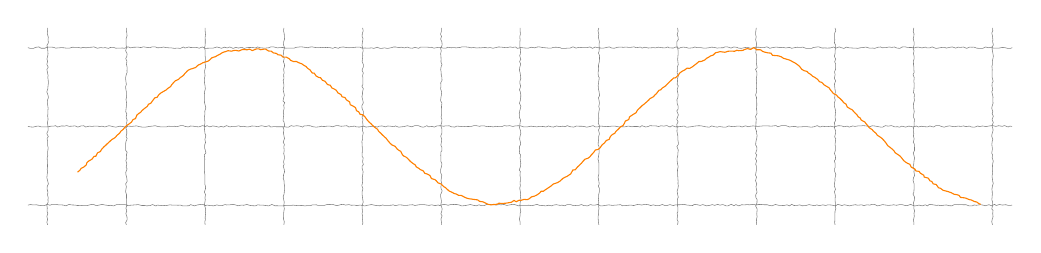
\begin{tikzpicture}[domain=-0.62:10.85,decoration={random steps,segment length=1pt,amplitude=0.3pt}]
    \draw[very thin,color=gray,decorate] (-1.25,-1.25) grid (11.25,1.25);
    \draw[color=orange,decorate] plot (\x,{sin(\x r)});
\end{tikzpicture}
\end{adjustwidth*}
\caption{This is a figure, simple and poorly drawn by my computer. The lines, intended to be physical representations of the glittering abstraction of pure length, have come out wobbly, like a plum pudding with too much plum. I will send my computer back to arithmetic class.}
\end{figure}

Aliquam in orci fermentum mauris auctor dapibus. Duis tincidunt tortor quis nunc iaculis dictum. Duis a eros consectetur, facilisis odio sit amet, gravida nunc. Nulla vel pretium arcu, nec luctus mi. Suspendisse iaculis magna at nibh ultrices faucibus. Nullam pellentesque velit sapien, sagittis molestie elit volutpat in. Suspendisse potenti. Integer felis enim, suscipit sit amet massa nec, aliquam tristique mauris. Praesent fringilla consequat lectus, a iaculis augue consequat vitae. Maecenas adipiscing porta scelerisque. Integer eleifend dui eu placerat varius. Nam a nunc quis odio hendrerit placerat id non elit. Mauris suscipit suscipit sapien, id ullamcorper arcu hendrerit faucibus.

\begin{knitrout}
\definecolor{shadecolor}{rgb}{0.969, 0.969, 0.969}\color{fgcolor}\begin{kframe}
\begin{alltt}
\hlkwd{library}\hlstd{(xkcd)}
\hlkwd{ggplot}\hlstd{()} \hlopt{+} \hlkwd{geom_point}\hlstd{(}\hlkwd{aes}\hlstd{(mpg, wt),} \hlkwc{data}\hlstd{=mtcars)} \hlopt{+}
  \hlkwd{theme_xkcd}\hlstd{()}
\end{alltt}
\end{kframe}

{\centering \includegraphics[width=\maxwidth]{figs/xkcd-1} 

}



\end{knitrout}

Sed vitae est auctor, malesuada est at, scelerisque ipsum. Donec vulputate auctor vulputate. Fusce vehicula dolor a interdum ornare. Suspendisse euismod dapibus nibh, a adipiscing magna rhoncus sed. Nulla ac quam urna. Mauris ornare elit non porta fermentum. Etiam elementum, lectus non vestibulum tempus, urna eros scelerisque metus, eget congue metus lorem ut lectus. Suspendisse id elit nec ipsum consequat rhoncus. Ut lectus mi, mollis eu quam vitae, posuere ullamcorper metus. Suspendisse non nisi vel nulla lacinia interdum.

Etiam fermentum augue et pulvinar ultricies. Aenean ut commodo enim. Ut vel turpis eu nisl sagittis facilisis. Nullam porttitor varius magna ac porttitor. Nunc eget augue dolor. Cras sagittis eget sapien at aliquam. Integer vel nunc quis lorem blandit congue. Fusce tristique volutpat leo, at lacinia purus ultricies ut. Nulla imperdiet odio at adipiscing ultrices. Morbi magna nisl, pretium mattis hendrerit vel, pharetra non risus. Proin egestas pharetra dolor, sed dictum nulla condimentum eu.

Cum sociis natoque penatibus et magnis dis parturient montes, nascetur ridiculus mus. Nunc quis sem ullamcorper tortor bibendum vestibulum lobortis ut justo. Maecenas eu lobortis felis. Cras in sagittis lacus. Ut quis laoreet risus. Etiam dui lectus, suscipit ut dui et, ullamcorper condimentum purus. Suspendisse volutpat ipsum metus. Curabitur tempus erat vel ante scelerisque varius.



\chapter{The Second Fascinating Fact}
This chapter is all about numbers (cf Table~\ref{tab:the-numbers}). Because, through hermetic machinations, these numbers reveal a hidden truth, we will discuss them in a dreamed language.

\begin{table}
\begin{tabular}{
    r
    S[table-format=1.3]
    S[table-format=3.5e-1]
    S[table-format=1.4]
    S[table-format=-1.5]
}\toprule
Frankness  & {$\aleph_0$} & {Widgets \& Bobbins} & {$\Delta_{\text{funk}}$} & {$r$}    \\ \midrule
Crows      & 5.897        & 0.3692               & 0.4679                   & -0.1367  \\ 
Malaise    & 5.128        & 1.692e-05            & 0.6395                   & -0.06257 \\ 
Lantern    & 6.334        & 0.7099               & 0.57                     & -0.1425  \\ 
Rushing    & 15.11        & 0.01569              & 0.3576                   & 0.01739  \\ \midrule
Splinters  & 3.753        & 1.084                & 0.2924                   & -0.1632  \\ 
Brilliant  & 3.174        & 1.061e+04            & 0.2827                   & -0.2533  \\ 
Still      & 3.192        & 1.795e+04            & 0.3066                   & -0.1173  \\ 
\midrule
Quickening & 2.93         & 250.6                & 0.999                    & -0.02164 \\ 
Barter     & 3.437        & 6.625e-06            & 0.8351                   & -0.6018  \\ 
Promise    & 9.753        & 16.03                & 0.5062                   & 0.1852   \\ 
\bottomrule
\end{tabular}

\caption{These are the numbers that this chapter is all about. As you can see, they are very interesting. Ponder.}
\label{tab:the-numbers}
\end{table}

Cras venenatis lorem quis mi luctus dignissim. Cras sed rutrum libero, ac auctor libero. Aliquam at aliquam nisi, at viverra justo. Donec lobortis fermentum suscipit. Ut quis mollis nibh. Aenean placerat ac leo a rutrum. Nam pharetra faucibus urna, vel ornare lectus convallis vitae.

Praesent dui purus, molestie et egestas vel, aliquam et lorem. Suspendisse accumsan tortor eu arcu pharetra consequat non non lacus. Aliquam erat volutpat. Donec sodales molestie mi vitae aliquam. Proin congue quis enim non interdum. Sed viverra, mi in pharetra pellentesque, quam mauris commodo lectus, nec ultricies diam mi eget nulla. Maecenas sodales interdum viverra. Mauris consequat orci id malesuada accumsan. Maecenas a ligula fringilla, placerat risus id, suscipit orci. Interdum et malesuada fames ac ante ipsum primis in faucibus. In hac habitasse platea dictumst. Nam nec sem tincidunt, posuere tortor ac, egestas arcu.

Donec non augue consequat, sagittis lectus in, varius massa. Aenean rutrum euismod ipsum. Nam at arcu neque. Sed leo metus, vestibulum non molestie vel, ultrices iaculis sem. Pellentesque sed pulvinar massa. Duis at placerat augue. Nunc quis nunc adipiscing, facilisis felis eu, eleifend ante.

Sed pharetra quam facilisis, rhoncus libero quis, elementum tellus. Etiam tellus massa, blandit a luctus nec, bibendum in ante. Phasellus porttitor, eros nec pulvinar commodo, erat orci ultrices erat, nec accumsan felis felis placerat lacus. In gravida dolor vel diam consectetur rutrum. Ut hendrerit ante ac aliquam aliquam. Mauris eleifend mauris ac orci lacinia lacinia. Interdum et malesuada fames ac ante ipsum primis in faucibus. Curabitur id tristique est. In vestibulum felis eu erat tempor semper. Vestibulum sollicitudin molestie purus non vehicula. Nunc eget aliquet metus. Nulla non ante ut nibh cursus feugiat.

Proin hendrerit vestibulum orci ut hendrerit. Sed ornare, magna et convallis euismod, nunc odio pharetra sapien, vitae ornare tellus eros sed magna. Nulla orci tortor, ultricies non orci convallis, mattis pharetra massa. Donec interdum justo id risus tincidunt auctor. Duis vulputate erat eros, eu varius eros lacinia nec. Fusce et gravida mauris, ut hendrerit odio. Quisque semper lacus lectus, id adipiscing risus facilisis at.

\section{A digression}
Nulla ut tempor orci. Praesent consequat sit amet elit nec volutpat. Mauris at nunc arcu. Proin luctus massa sed sapien pretium porta nec vel dolor. Mauris non dui eros. Pellentesque mollis fringilla dui, vel congue dolor dapibus nec. Nam sollicitudin odio tortor, et dictum dolor bibendum nec.

Sed malesuada urna augue. Mauris vestibulum lectus ipsum, dignissim auctor nisi imperdiet at. Vestibulum facilisis iaculis felis, quis scelerisque odio sagittis id. Nunc non sapien lacinia, fermentum dui non, sagittis augue. Ut non nisi consectetur, hendrerit odio quis, tincidunt ante. In lacinia elit sed ligula elementum, vitae consequat neque pulvinar. Cum sociis natoque penatibus et magnis dis parturient montes, nascetur ridiculus mus. Etiam porta quis libero sit amet venenatis. Curabitur quis interdum lorem, in eleifend dui. Donec in arcu sodales, vehicula ipsum fermentum, pharetra nibh. Sed porttitor elit vel orci eleifend elementum. Integer aliquet arcu quis nunc facilisis malesuada. Praesent at nisl felis.

\subsection{Point}
Mauris tristique tortor a gravida cursus. Sed non urna a mauris fringilla ullamcorper. Praesent commodo urna nec elit elementum, vel tincidunt mi blandit. Pellentesque habitant morbi tristique senectus et netus et malesuada fames ac turpis egestas. Praesent lectus mauris, fermentum non arcu nec, fermentum lacinia libero. Maecenas vitae hendrerit massa. Curabitur pharetra ipsum ut ligula tempus, ac commodo justo laoreet. Cras viverra, orci at dapibus blandit, massa lacus tincidunt leo, laoreet dictum justo libero eu tortor.

Proin tincidunt justo fermentum dignissim accumsan. Cras porttitor orci nunc, nec fringilla mauris posuere vel. Curabitur mi mi, aliquam ac lectus sit amet, blandit euismod nulla. Maecenas sollicitudin fringilla dignissim. Aliquam erat volutpat. Aliquam at elementum arcu, quis scelerisque orci. Integer ultrices, nisl sit amet sagittis posuere, erat odio tincidunt justo, eu porttitor sapien risus vitae risus. Quisque id nibh sollicitudin, aliquet risus at, semper elit. Donec porttitor arcu eu diam placerat, sit amet blandit tellus gravida. Aliquam ornare vitae libero vitae mollis. Sed ante leo, venenatis nec felis sed, semper adipiscing ipsum. Vivamus et pulvinar nibh. Mauris viverra tortor vitae lacus ullamcorper, in iaculis sapien egestas. Donec dapibus in odio at tempus. Nulla laoreet, metus ac dapibus euismod, leo arcu gravida massa, nec adipiscing lorem urna a risus.

\subsection{Counterpoint}
Nam vitae porta ante, vitae tincidunt sapien. Fusce scelerisque arcu sem, nec facilisis nisi commodo porta. Etiam vulputate sed enim eu vestibulum. Donec placerat est id elit elementum ultricies. Ut arcu lorem, iaculis nec odio ut, porta pharetra ante. Sed metus purus, lacinia nec mattis et, placerat sed sem. Integer rutrum consequat nulla, id consectetur tortor scelerisque nec. Integer nec odio suscipit, tincidunt elit at, cursus enim. Curabitur id aliquam dui, quis porttitor risus. Ut commodo risus quis posuere adipiscing. Sed eget ipsum sapien. Donec lacinia elit hendrerit euismod euismod. Fusce semper quam ut lorem venenatis accumsan. Duis posuere, urna quis mollis tristique, metus tellus laoreet nunc, et vestibulum sapien nulla sed neque.

In ut nisl vestibulum, tincidunt enim et, lacinia ante. Praesent feugiat nibh sem, vel porttitor nunc auctor vitae. Suspendisse dictum, lorem nec pulvinar auctor, dui mi vulputate ligula, tincidunt faucibus odio eros vel orci. Praesent vitae adipiscing urna, nec tristique nulla. Fusce bibendum quis ipsum eget aliquam. Donec pretium nisi eu tortor varius, mollis dignissim eros viverra. Nulla vulputate facilisis magna et egestas. Nullam facilisis nec libero ut adipiscing. Phasellus mollis tellus nec urna ornare euismod.

Aenean ut eros lorem. Lorem ipsum dolor sit amet, consectetur adipiscing elit. Mauris pretium, mauris vel volutpat volutpat, diam ipsum suscipit ante, vel semper lacus enim in felis. Nullam viverra pharetra tincidunt. Fusce metus purus, molestie et risus eu, interdum sollicitudin risus. Nulla pretium augue a mi faucibus congue. Vivamus risus diam, pulvinar sit amet sagittis eu, vulputate et ipsum. Nam vitae fermentum lectus. Curabitur nec malesuada risus. Vestibulum enim felis, scelerisque a pellentesque ut, vestibulum eu risus. Nulla dictum metus quis nisl aliquet semper. Etiam in laoreet augue. Donec tempor, tellus vel eleifend placerat, libero diam placerat mauris, sed fermentum mauris nunc eget diam.

\subsection{Harmony}
Interdum et malesuada fames ac ante ipsum primis in faucibus. Aenean viverra pulvinar magna, a blandit arcu accumsan vel. Donec auctor nisi in dolor ornare, in dapibus lacus aliquam. Maecenas quis risus in nisi placerat commodo ac at dui. Integer porta, odio ut ultricies varius, urna neque accumsan odio, id suscipit quam magna non sapien. Mauris viverra justo id orci congue, tincidunt ullamcorper lacus adipiscing. Aenean laoreet convallis diam nec scelerisque. Fusce cursus, purus lacinia venenatis mollis, magna lectus lacinia eros, at posuere enim ante at ligula. Suspendisse in scelerisque metus, nec auctor arcu.

Fusce eleifend ultrices libero. In semper, risus eget euismod feugiat, quam metus ultricies nunc, in dapibus velit sem at neque. Maecenas at nunc vel nisl elementum cursus sit amet eget arcu. Praesent ultrices, arcu id facilisis consectetur, nunc enim convallis nunc, nec aliquam mauris ligula in magna. Nunc quis nunc leo. Nulla in enim eget tellus aliquet iaculis. Phasellus suscipit ante vel accumsan lobortis. Sed sit amet scelerisque magna. Nam vulputate est et sapien tristique fermentum. Duis vel dignissim erat. Nullam auctor nisl a nulla pellentesque, consectetur volutpat turpis ornare. Mauris fermentum pretium risus, non euismod nibh mattis in. Sed vulputate, purus vitae mattis pretium, erat justo sagittis nulla, quis rutrum ligula metus eget odio. Fusce vel nunc scelerisque risus lacinia consectetur id semper odio. Vivamus fringilla arcu id eros pretium, pellentesque porta dui porta.

Nulla sollicitudin ut orci sit amet laoreet. Aliquam eu sem in leo hendrerit venenatis sit amet mattis justo. Fusce adipiscing euismod libero at dignissim. Vivamus laoreet nisi vitae tellus porttitor vulputate. Praesent a pellentesque dui. Vivamus facilisis tellus sem, ac dictum magna hendrerit at. Pellentesque at ipsum at ante fringilla sodales ac in arcu. Ut ut rutrum turpis, et dapibus magna. Sed metus eros, interdum tempus suscipit nec, condimentum a nunc. Sed non quam vel dui scelerisque porttitor sit amet quis ipsum. Integer mauris orci, ultrices a neque ac, vestibulum placerat odio. Nunc metus lectus, fringilla vel nulla sit amet, mollis ornare diam.

\section{A regression}
Cras aliquam molestie dui, non venenatis nulla consectetur et. Nulla convallis diam dui, nec tristique ligula volutpat sit amet. Cras quam erat, faucibus eu feugiat in, dignissim at diam. Duis sit amet lectus in lorem faucibus tincidunt ac vitae eros. Cras tristique fermentum lorem sollicitudin dignissim. Donec feugiat felis porttitor lorem volutpat, at tristique ante ultricies. Maecenas tellus massa, scelerisque at dolor a, tempus tempor urna. Praesent sodales congue sem id interdum.

Vestibulum vel orci eu lectus luctus vestibulum non at lectus. Pellentesque habitant morbi tristique senectus et netus et malesuada fames ac turpis egestas. Phasellus euismod adipiscing hendrerit. Donec eu tempor odio. Suspendisse orci risus, aliquam sit amet adipiscing nec, sollicitudin in purus. Maecenas malesuada laoreet nunc eu feugiat. Nullam fringilla convallis adipiscing. Donec et sem dolor. Proin commodo pharetra leo vel semper. Phasellus posuere massa sed imperdiet vestibulum. Ut ultrices pulvinar leo id hendrerit. Pellentesque volutpat eu libero vitae lobortis. Mauris cursus sem mauris, vel mollis lacus elementum quis.

Morbi ullamcorper, nisi eget tempor venenatis, orci nisl ultrices est, nec eleifend ante neque id ligula. Vestibulum ut purus ut metus ornare pretium. Vestibulum eleifend, urna sit amet semper consectetur, arcu nibh fringilla velit, a aliquet enim erat in arcu. Nam tincidunt sapien in ipsum hendrerit, id ornare massa laoreet. Sed ultrices lorem ac egestas sagittis. Integer aliquet imperdiet elit, convallis lacinia dolor consectetur eu. Nam lacinia quam magna, at fringilla elit egestas id. Integer eget felis ac quam blandit fringilla vel at tortor. Vivamus pulvinar hendrerit enim et vehicula. Pellentesque tempor tristique enim, vitae blandit sem consequat vitae. Aliquam fringilla vehicula arcu. Praesent erat nunc, ornare sit amet tempus nec, facilisis ac dui. Phasellus vestibulum dui orci, quis volutpat neque vulputate eu.

\begin{equation}
E = m \sqrt{c}
\end{equation}

Maecenas ligula tellus, consequat vitae lacus et, malesuada lobortis diam. Vestibulum ultricies convallis lacus, tempor ullamcorper arcu faucibus id. Quisque consectetur nisl nec risus tincidunt tristique. Etiam vel dolor mattis, facilisis tellus ac, convallis elit. Phasellus volutpat posuere metus id placerat. Sed nisi mi, egestas quis lacus eu, vulputate vulputate arcu. Aliquam sed mauris bibendum, laoreet nibh at, volutpat diam. Ut dapibus euismod arcu. Duis tincidunt placerat metus et ultricies. Duis eget vehicula est, ac hendrerit lorem. Morbi tincidunt molestie dui vitae luctus. Aliquam eu lacinia lacus. Nulla non ornare elit. Fusce cursus rutrum lorem, vel venenatis orci scelerisque ac. Aenean quis pretium massa, in pellentesque metus.

In tincidunt nibh vel nisi pharetra egestas. Praesent lectus lacus, ultrices a venenatis sed, vestibulum sagittis est. Maecenas diam tellus, porta vitae ipsum sit amet, suscipit hendrerit orci. Integer cursus tincidunt urna. Vivamus non tristique mauris, vulputate volutpat massa. Maecenas lorem nisi, feugiat eget pharetra tristique, mollis a justo. Interdum et malesuada fames ac ante ipsum primis in faucibus. Pellentesque euismod, lorem a euismod tempus, sem risus fringilla tellus, sed porta sem eros non nibh. Curabitur aliquam lectus vitae orci scelerisque, sed ultricies justo pretium. Praesent sed metus urna. Sed risus elit, dignissim sit amet tristique et, iaculis ac leo.

Cras eget pellentesque orci. Donec eget placerat est. Suspendisse vitae massa sodales, semper odio vitae, faucibus nisi. Cras faucibus hendrerit adipiscing. Fusce euismod bibendum consectetur. Aenean pellentesque in quam ac ornare. Pellentesque tristique nunc mauris, nec mattis lectus varius sit amet. Sed blandit ipsum enim, in condimentum est lacinia vitae. Etiam metus eros, pellentesque ac auctor id, congue id ipsum. Phasellus hendrerit ante quis velit viverra, ut ultrices ipsum convallis.

Morbi eget quam tincidunt, congue velit at, placerat metus. Fusce pulvinar aliquam venenatis. Maecenas sed aliquet lectus. Pellentesque varius quam vitae posuere sollicitudin. Maecenas sed nisi urna. Fusce sed sollicitudin mauris, sed varius eros. Vestibulum vulputate vehicula massa sit amet commodo. Morbi pulvinar sem ut auctor ornare. Curabitur pretium pulvinar elit nec ornare. Phasellus ultricies leo elementum velit semper, et lobortis libero semper. Etiam quis euismod erat. Maecenas hendrerit, ligula ut vestibulum placerat, mauris velit dapibus elit, ut viverra metus nunc pretium ante. Curabitur id felis eu erat facilisis egestas lacinia ut mauris. Etiam sed nibh euismod erat consectetur elementum consectetur non lorem. Suspendisse malesuada ut risus non sagittis.

\section{A plaintive call for humanity}
Cras sollicitudin feugiat erat a gravida. Sed non nulla quis felis iaculis aliquam. Morbi congue, justo non blandit auctor, augue turpis venenatis massa, in gravida lacus sem vitae turpis. Nulla semper, neque in mollis dignissim, quam felis aliquam libero, dictum semper nisl tellus vel mauris. Nam aliquet molestie eros, quis venenatis metus imperdiet nec. Nunc nec consectetur urna. Donec vitae erat eu nunc lacinia vulputate sit amet quis libero. Nunc feugiat in ante iaculis tincidunt. Pellentesque non gravida magna, non pulvinar mauris. Nullam consectetur quam sit amet est elementum sollicitudin.

Pellentesque vitae sollicitudin mi. Mauris diam elit, ultricies ut tristique eget, viverra vitae ligula. Curabitur scelerisque eleifend eros vel aliquet. Phasellus auctor, tortor a accumsan aliquet, diam mauris gravida lectus, vel congue sapien ipsum id ligula. Quisque eget rhoncus quam. Nullam et sem iaculis, dictum eros viverra, facilisis justo. Maecenas in libero lectus. Nullam vel ornare dui. Integer at velit ipsum. Nunc lobortis tempus nulla, ut aliquam velit laoreet vitae. Sed quis dapibus augue, vel convallis justo. Donec ac pharetra velit. Cras vel risus ut lorem sollicitudin vestibulum ut ac lacus. Suspendisse potenti. Cras luctus mi vitae pellentesque scelerisque.

Vestibulum semper placerat lectus, sed laoreet elit malesuada a. Aenean accumsan, nulla blandit facilisis feugiat, risus quam posuere enim, auctor volutpat diam magna id tellus. Suspendisse eu accumsan sapien, sed vehicula risus. Proin a eros sit amet risus rutrum vulputate. Integer dui est, vulputate eget lacus nec, rutrum iaculis sem. Mauris fermentum lectus nec sem euismod, sit amet tempus enim sodales. In sit amet condimentum sem, at ornare purus. Ut eget tristique nisl. Sed blandit, orci quis lacinia gravida, ante magna dapibus orci, vel scelerisque elit lacus quis arcu. Morbi at rutrum velit.

Praesent ac metus condimentum, semper lectus ut, luctus dolor. Sed semper ipsum turpis, nec rhoncus enim dapibus ac. Praesent eu ornare eros, quis suscipit neque. Donec at nisi posuere, rutrum diam ac, ornare est. Duis adipiscing pretium mollis. Maecenas pellentesque nunc sed tellus vulputate lacinia. Proin nec ante laoreet, lobortis diam eu, dapibus tellus. Donec ultricies nulla magna, nec posuere nunc pretium id. Nulla eu massa ut nisi imperdiet ultricies. Quisque placerat eros justo, in accumsan nisl rhoncus nec. In volutpat non leo sit amet ultricies. Pellentesque nec semper leo. Nulla sit amet arcu vel risus porttitor malesuada.

Pellentesque habitant morbi tristique senectus et netus et malesuada fames ac turpis egestas. Aliquam dapibus rutrum egestas. Integer nec pharetra tellus, non vestibulum mi. Proin ornare ligula velit. Vivamus est libero, aliquam quis tristique et, sodales in enim. Sed placerat arcu erat, et eleifend nisi ultrices ut. Ut aliquet pulvinar turpis, non iaculis enim tempus ac.

Cum sociis natoque penatibus et magnis dis parturient montes, nascetur ridiculus mus. Mauris at tellus lorem. Sed mauris nunc, mollis eu velit eu, dapibus faucibus diam. Ut ultricies laoreet posuere. Nam malesuada condimentum quam vitae eleifend. Proin venenatis placerat massa, sed tempus libero adipiscing at. Nulla non urna accumsan, accumsan urna vel, lacinia mi. Sed a scelerisque odio. Ut at ullamcorper urna, ultrices sodales metus. Nullam nulla ante, tempus non dictum blandit, mollis nec elit. Nam ullamcorper enim ipsum, id sodales purus aliquam vitae. Phasellus nunc metus, ultricies eu tempor vel, rhoncus eu tortor. In luctus quam et congue laoreet.

Nam libero dolor, euismod non lorem eu, consectetur feugiat dui. Nunc erat ligula, vestibulum eu tellus at, ultricies egestas urna. Nam dapibus consequat mauris sit amet condimentum. Donec quam lorem, pretium vitae nisl et, posuere varius tortor. Duis ultricies orci ut arcu suscipit, eget tempor nisl sollicitudin. Donec sit amet aliquam libero, vitae rhoncus magna. Ut elementum odio sed tempus rhoncus. Cras sagittis eu tortor sed dictum. Aliquam erat volutpat. Vestibulum quis est vitae justo semper malesuada. Vivamus varius pulvinar iaculis. Nunc fringilla augue risus, sit amet rutrum augue eleifend sit amet. Cras quis volutpat erat, ac luctus urna. Aliquam molestie tortor interdum tortor porta tincidunt. Proin vitae iaculis orci. Vivamus erat lectus, consequat viverra urna non, dignissim semper purus.

Etiam porttitor lacus orci, non eleifend risus ornare ac. Vestibulum ultrices lectus volutpat congue molestie. Etiam bibendum nulla varius, vestibulum metus sit amet, vestibulum nisl. Fusce facilisis odio nisi, ut suscipit mauris porttitor at. Maecenas quam purus, fermentum sed turpis id, iaculis vulputate augue. Vestibulum porttitor quam venenatis placerat facilisis. Aliquam vel rutrum diam. Donec malesuada commodo vestibulum. Mauris quis mauris venenatis, pulvinar tellus non, gravida tortor.

Morbi vulputate non nulla eu sollicitudin. Quisque dictum diam porttitor vehicula suscipit. Phasellus vitae mi congue, ornare magna vel, convallis libero. Nullam non vehicula nunc. Phasellus fringilla, lacus id malesuada viverra, lacus turpis aliquam ligula, non adipiscing enim leo sit amet ligula. Phasellus faucibus ante nulla, ac malesuada est ornare et. Pellentesque dictum tellus et ligula tempor interdum. In ornare massa mi, in vehicula justo sodales id. Ut dignissim pretium purus, sit amet aliquet risus tristique et. Vivamus viverra arcu ut mauris euismod ultricies. Fusce tortor velit, gravida consequat urna at, ornare porttitor sem.

Aliquam ut risus a urna vestibulum lobortis vel sit amet magna. Nam et elementum nulla, non dictum nisl. Suspendisse potenti. Nulla fermentum est leo, et scelerisque nulla accumsan ut. Nam interdum lorem eget rutrum molestie. Vivamus bibendum, risus in aliquam malesuada, dui est porttitor arcu, at tempus nisi magna et augue. Nulla convallis condimentum massa, et dignissim nisl bibendum sed. Maecenas ac nunc tempor, porttitor lorem sit amet, posuere sem. Integer gravida lorem nec tincidunt ultrices.

Proin porta tincidunt ligula. Donec varius metus et felis tincidunt, pharetra volutpat nisi lacinia. Quisque id massa velit. Nam non justo quis est imperdiet gravida. Ut luctus ornare nisl, eget placerat neque congue quis. Donec massa eros, gravida eu nibh id, condimentum bibendum tortor. In sollicitudin mauris eget nisl bibendum, ut suscipit lacus sollicitudin. Phasellus rhoncus venenatis mauris, et scelerisque neque sagittis gravida. Nam sodales, nisi ut aliquet fringilla, felis augue ultricies ante, non consequat nibh nunc eu mauris. Donec eu arcu odio.

Sed dapibus non leo eget porta. Nunc a justo enim. Nam non fermentum elit. Integer in nulla turpis. Ut facilisis, purus ut varius hendrerit, magna augue aliquet nisi, eget varius urna ante sed nulla. Vestibulum ac eros lorem. Etiam imperdiet nibh eu tempus semper. Donec venenatis non orci eu lacinia. Nunc feugiat tellus est, et dictum odio vehicula a. Quisque sagittis tempor ultrices. Sed accumsan sollicitudin arcu, quis auctor dui auctor sed. Aliquam et ligula leo. Sed bibendum enim quis varius egestas. Sed feugiat ipsum purus, eget ullamcorper massa dictum ut. Ut semper lorem lectus, a pretium libero pharetra ac.

Donec et magna pharetra, consequat magna ut, egestas lorem. Etiam egestas ornare mi, vitae aliquam orci tincidunt nec. Donec sit amet leo nisi. Aliquam quis odio convallis, ullamcorper risus quis, ullamcorper mi. Vestibulum tincidunt semper vulputate. Lorem ipsum dolor sit amet, consectetur adipiscing elit. Proin nec dui bibendum, aliquet sem ut, blandit nibh.

Maecenas tincidunt sem a turpis vestibulum, quis ultrices dui feugiat. Duis mauris purus, elementum id ipsum ac, laoreet tristique eros. In suscipit sed justo nec consequat. Vestibulum aliquam malesuada tristique. Cum sociis natoque penatibus et magnis dis parturient montes, nascetur ridiculus mus. Sed blandit nunc eget purus tempor convallis. Vestibulum fringilla cursus est, eu posuere mi hendrerit et. Etiam ac elit imperdiet, lobortis nibh id, faucibus nulla. Nullam ullamcorper urna est, vestibulum porta metus consectetur nec.

Mauris suscipit elit orci, sed dictum elit adipiscing sit amet. Sed suscipit, magna ac hendrerit imperdiet, quam dui dapibus erat, in tristique enim quam non velit. Sed non accumsan ante. Proin eget sagittis ante. Class aptent taciti sociosqu ad litora torquent per conubia nostra, per inceptos himenaeos. Nullam elementum lorem id purus rhoncus sagittis. Etiam eleifend diam tincidunt, vulputate risus ac, interdum eros. Vivamus vitae porttitor sapien. Vestibulum odio dolor, facilisis nec malesuada blandit, condimentum sit amet odio. Ut vestibulum ante et molestie euismod. Vivamus et dictum mauris, eu venenatis lacus. Suspendisse sodales commodo dapibus. Donec quis ligula sed justo tempor pretium. Curabitur quis aliquam nisl.

Vestibulum venenatis, nisi at laoreet pulvinar, nibh mi dapibus lectus, nec consequat leo lectus ultricies quam. Sed id nunc ut sem imperdiet adipiscing. Etiam eros diam, malesuada placerat semper ac, semper non nulla. Aenean nec odio sit amet purus fringilla mollis. Cras malesuada eget massa at ultrices. Pellentesque venenatis nibh ut lacus fringilla, non placerat erat tincidunt. Phasellus non mauris vitae ante dignissim consequat. Vivamus et libero magna. Nullam in quam sed mauris cursus egestas ut sit amet ante. Maecenas augue neque, faucibus vitae tincidunt eu, condimentum sed erat. Curabitur lobortis dolor at tellus cursus sollicitudin. Integer vehicula molestie ante, ac molestie enim vestibulum id.

Integer ac fringilla purus. Pellentesque dapibus dignissim augue vel mattis. Donec sed suscipit purus, vitae pulvinar eros. Sed at metus id eros aliquet dignissim varius sit amet metus. Etiam felis mi, porttitor non tincidunt in, fermentum sit amet metus. Sed fermentum ligula eget tellus laoreet interdum. Sed id nunc eget arcu imperdiet aliquet. Etiam at iaculis libero. Sed scelerisque massa in placerat molestie. Integer convallis pulvinar nisi, eget egestas sem condimentum ac. Sed sed ipsum quis tellus accumsan placerat. Nunc ultricies orci massa, a tristique sapien bibendum id.

\end{document}
